\chapter{3D musical instruments and 3D displays for performance}
\section{Subject presentation}
\paragraph{3D Musical instruments}
At the \ac{SCRIME} and \ac{LABRI}, three-dimensional musical instruments have been implemented within the context of research in interactive virtual reality and music computing. 

The \brand{Drile} \cite{berthaut2010drile} is a 3D musical instrument which allows manipulation of the structure of a song using \gls{livelooping}, in an immersive virtual reality scene.

The \brand{Aerial Percussion} is a 3D musical instrument which generates sounds using the position in space of sensors which are put at the end of drumsticks. Virtual 3D shapes like cubes, cylinders, are positionned around the instrument and the musician. According to the position, the orientation, and the speed of the sensors, sounds are generated.

\paragraph{Required work}
We were asked to implement a prototype of a 3D render and display device, for musical performance.
It is necessary to take into account the constraints inherent to a musical performance environment, as well as the constraints of the instruments.

Here are some constraints for the performance : 
\begin{itemize}
\item The musician has to be in front of the audience.
\item The musician requires visual cues inherent to the utilisation of the instrument, and the audience must see the instrument to understand the gestures and actions of the musician.
\end{itemize}

To enact this implementation, a precise explanation of the nature of the 3D musical instruments is required.

\paragraph{Plan for this section}
We will first make a short presentation of 3D musical instruments, present and will then define the concepts of immersivity and interactivity.

\newpage
\section{What is a 3D musical instrument?}
{\LARGE{TODO a reformuler : bof le wikipédia}}\\
A 3D musical instrument, or an immersive virtual musical instrument, represents sound processes and their parameters as 3D entities of a virtual reality so that they can be perceived not only through auditory feedback but also visually in 3D and possibly through touch as well as haptic feedback, using 3D interface metaphors consisting of interaction techniques such as navigation, selection and manipulation.

\paragraph{Example for the Drile}
For instance, the picture \ref{drile} shows a musician with special glasses, as well as joysticks with force-feedback haptic sensors (Piivert \cite{berthaut2010piivert}). 
The user handles 3D shapes in a 3D environement to influence the music generation. A specific part of this report will be dedicated to a precise study of the \brand{Drile}.

\begin{figure}[t]
\centering
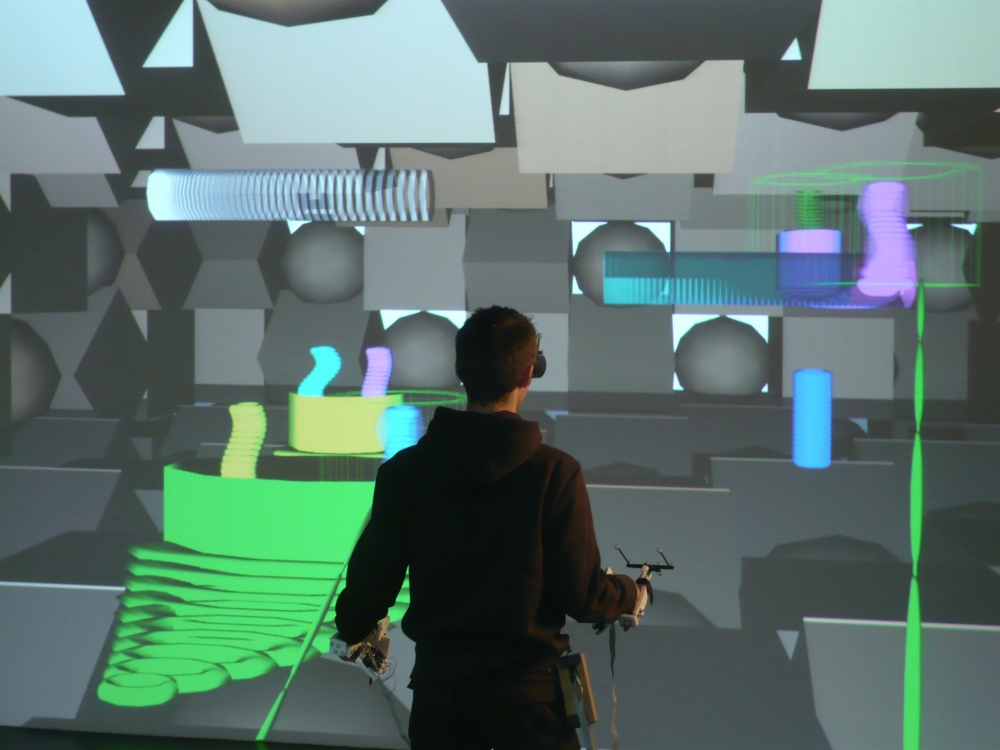
\includegraphics[scale=0.3]{image/drile.jpg}
\caption{Picture of a musician using DRILE}
\label{drile}
\end{figure}

\newpage
\section{Immersion}
\paragraph{Definition}
Immersion is a psychologic state where the subject stops about taking care of its own physical state.
The immersion is quite important in virtual reality. For instance, for the Aerial Percussion, it would come down to the state the performer is when he stops thinking consciously of the disposition of the shapes he interacts with. The musician will then be immersed in the virtual 3D environment which consists in the shapes disposition.

\paragraph{}
Hence, to immerse an user, multiple parameters are accessible to the 3D instrument designer. 
They are mostly linked to the senses of the human body. In our project, we will mainly focus on vision, and more precisely on 3D display devices.

\paragraph{}
Interactivity is an important aspect of the immersion capacities of a musical system.
The user is more likely to get an immersive feeling in a virtual world, if the world instantly reacts to his actions
L'interactivité a une part importante dans l'aspect immersif d'un système. L'utilisateur a d'autant plus le sentiment d'immersion dans un monde virtuelle si celui ci réagit instantanément à ses actions. Ceci nous amène a définir les contrôles d'un instrument de musique 3D et l'importance de l'interactivité.

\section{Control}
\paragraph{}
Pour le contrôle de l'instrument de musique 3D, il est important de voir le système de deux manières. Dans un premier temps comme un instrument de musique, qui donc doit répondre à certaine contraintes qui permet d'assurer la précision et la qualité attendu par un musicien de son instrument. Et dans un second temps comme un système interactif immersif, c'est à dire une très grande interactivité et de tirer profits un maximum des caractéristiques de l'être humain (retour visuelle immersif et retour haptique).

\paragraph{}
Pour la manipulation d'un instrument de musique, la segmentation de la gestuel faite par Cadoz \cite{cadoz1999musique} est très pertinente. Cadoz définit trois types de gestes:

\begin{itemize}
\item les gestes de sélection : action de sélection du musicien d'un composant de l'instrument plutôt qu'un autre, par exemple dans le cas d'un violon cela revient à choisir une corde plutôt qu'une autre.
\item les gestes de modification : action qui modifit l'état de l'instrument, dans le cas d'une guitare cela revient à utiliser sa main gauche pour presser une ou des cordes sur l'une des cases du manche.
\item les gestes d'excitation : action qui génère directement et physiquement le son, qui revient à pincer une corde dans le cas d'une guitare. C'est ce geste qui est soumis à l'expression de l'artiste.
\end{itemize}

\paragraph{}
Mais il ne faut pas oublier le caractère immersif du système, celui impose que l'utilisateur ait un certain confort de manipulation. L'immersion visuelle est souvent améliorer grâce à un suivi de tête à l'aide d'une Kinect. Ceci permet d'adapter la projection en fonction de la position de la tête de l'utilisateur et cela augmente l'impression d'immersion.
Des boutons de pressions à retour haptique augmentent aussi la conscience des actions de l'utilisateur, donc sa précision d'action.

\paragraph{}
Nous verrons dans la suite de ce rapport que Florent Berthaut s'est posé toutes ces questions lorsqu'il a conçu Piivert \cite{berthaut2010piivert} pour contrôler le DRILE.

\paragraph{}
Maintenant que le concept d'instrument de musique 3D est bien défini, nous allons pouvoir nous focaliser sur les techniques de rendu 3D qui nous intèressent plus particulièrement vis à vis de notre sujet.

